% ==============================================================================
% 第 3 章：如何设计程序 (Chapter 3: How to Design Programs)
% ==============================================================================

\chapter{如何设计程序}
\label{sec:ch03_htdp}

本书前两章表明，学习编程需要掌握诸多核心概念。一方面，编程需要一门语言作为媒介，以此准确表达我们希望计算机执行的计算。用于表述程序的计算机语言是人工构建的符号系统，但掌握一门编程语言与掌握一门自然语言在很多方面有相通之处：二者都包含词汇、语法以及对“语句片段”所代表含义的理解。

另一方面，至关重要的是学会\textbf{如何从问题陈述一步步走向最终程序}。我们需要从自然语言的题目中辨别出哪些信息是关键核心，哪些细节可以暂时忽略；我们需要抽丝剥茧，理清程序接收什么输入、产出什么输出，以及输入与输出之间存在怎样的对应规律；我们需要了解并确认所选用的语言及其内置库是否已经提供了处理这些数据所需的基础操作——若未提供，我们必须有能力构思并实现相应的辅助函数；最后，当代码写完后，我们必须严格检验它是否确实完成了预期的计算，并在发现各色各样的缺陷时，能够从容理解并修复它们。

所有这一切听起来颇具挑战，你可能会纳闷：为什么我们不直接“摸着石头过河”，随性写写改改、到处试试，只要凑出看起来还不错的输出结果就收工大吉？这种常被称为“车库式编程”（garage programming）的随性方式极为普遍，且在许多场合确能取得暂时的成功；它甚至往往是许多初创公司的起步摇篮。然而，初创公司绝无法直接将这种粗糙的“车库产物”作为可靠产品推向市场，因为除了最初的作者及其亲近的朋友，外人根本无法理解、使用和维护它。

一个优秀的程序必须配备简明扼要的说明文档，清晰阐述它的功能职责、期望接收的输入类型以及产出的输出规格。理想情况下，它还应自带一套可自动验证其正确性的证据体系。在最理想的工程状态下，程序代码与原始问题陈述之间的映射关系应当一目了然，从而使业务需求上的微小变动能够轻而易举地映射为程序代码中的微小调整。软件工程师将这种严谨的工业级成品称为\term{编程产品}（programming product）。

这一切看似额外的严谨工作之所以不可或缺，是因为\textbf{程序员从来不是只为自己写代码}。程序员写出的代码是给其他程序员阅读的，而在特定的时刻，人们会运行这些代码来解决现实问题。绝大多数现实程序都是由成百上千个函数协同协作的庞大系统，没有任何人能在一天之内独立写完所有模块。工程师加入项目团队、编写代码、随后离开；新的维护者接手遗留系统并继续演进。另一个无法回避的现实是：客户对业务需求的理解往往是动态变化的，他们最初提出的需求通常只说对了大半，细节上往往错漏频出。更糟糕的是，程序作为高度复杂的逻辑构造体，不可避免地会受到人类思维盲区的影响——简言之，程序员必定会犯错。终有一天，潜在的缺陷会暴露出来，工程师必须回过头来，重新研读一个月前、一年前、甚至二十年前写下的代码并进行修正。

\begin{notebox}[重读代码的现实]
这里所说的“其他程序员”，也包括“未来的你自己”——数月之后的你通常早已记不清当初年轻的自己在编写这段代码时脑海中的全部推导细节。
\end{notebox}

\begin{exercise}{千年虫（Y2K）问题调研}{33}
通过查阅资料，调研 20 世纪末震惊全球的“2000 年问题”（又称千年虫问题，Y2K problem）。了解当时的程序员为何采用两位数字来表示年份，以及这一历史设计决策在数十年后给全球银行业、航空业及各工业系统造成了何种深远的技术与经济冲击。
\end{exercise}

为了帮助所有人摆脱盲目摸索的泥潭，我们在此隆重推出\term{程序设计配方}（Design Recipe）。它将系统化的分步推导过程与以问题数据为核心的程序组织结构紧密熔铸为一体。对于那些一面对着空白屏幕就陷入焦虑发呆的读者，这套设计配方提供了一条有章可循、步步为营的确定性路径；对于从事编程教学的教师，它是诊断初学者思维卡点的精准试金石；对于从事医学、新闻或工程等其他领域的专业人士，这套科学严谨的问题解决范式同样能够跨界迁移；而对于立志成为一流软件架构师的读者，设计配方更是深入剖析并驾驭现有复杂大型软件的无上利器。

本章的剩余部分将带你迈出踏入设计配方世界的第一步；在后续各章节与各部分中，我们将在此基础上不断对该配方进行迭代深化与拓展。


% ==============================================================================
% 3.1 设计函数
% ==============================================================================
\section{设计函数}
\label{sec:3.1}

\subsection{信息与数据}

程序的终极目的，是描述一个消费现实\term{信息}（information）并产出全新信息的计算过程。从这个意义上说，程序类似于数学老师向小学生布置的解题指令。但与学生不同的是，程序处理的对象远不仅限于数字：它计算导航路线、检索联系人地址、操控物理开关、或者维护电子游戏的世界状态。所有这些信息均来源于现实世界的某一特定领域——通常被称为程序的\term{业务领域}（domain），而程序计算产出的成果则代表了该领域中的新信息。

“信息”在我们的设计哲学中居于中枢地位。可以将信息视为关于程序业务领域的具体事实。对于一个家具目录管理系统，“五条腿的桌子”或“两米乘两米的正方形桌子”都是信息。游戏程序面向不同的业务领域，其中的数值“5”可能代表游戏角色在屏幕上每个时钟周期移动的像素位移。而在薪资结算系统中，“5”可能代表“五项税前扣除”。

为了让程序能够处理现实信息，它首先必须将信息转化为编程语言内部的某种\term{数据}（data）；随后对这些数据执行计算；计算完毕后再将产出的数据还原解释为现实信息。对于交互式程序，这三步可能交替穿插、往复循环：根据需要随时从外部世界捕获更多新信息，并在计算间隙持续向现实世界反馈信息。

我们之所以选用 BSL 语言与 DrRacket 环境，正是为了让你在起步阶段完全不必为“信息与数据之间复杂的底层编解码”分心劳神。在 DrRacket 中，你可以直接把函数应用到核心数据上并直接观察其产出。这样就巧妙避开了“既要写业务计算、又要写复杂数据解析器”的鸡生蛋蛋生鸡困境。对于简单形态的信息，编写转换代码尚属简单；但对于复杂信息，你需要深入掌握语法解析（parsing）等高阶技术，而这需要非常扎实的程序设计功底作为前提。

软件工程界常用\term{模型--视图--控制器}（MVC）这一经典架构模式来概括这种分离：BSL 与 DrRacket 将底层纯数据处理与外部界面的信息解析和呈现彻底解耦。现代高质量软件工程已经形成共识：优秀的系统必须严格执行这种分层解耦，哪怕许多入门书籍仍然将二者混为一谈。依托 BSL 和 DrRacket，你可以心无旁骛地专注于程序核心计算逻辑的设计；当你在核心设计上积累了足够的经验之后，再自如地进阶学习信息与数据双向转换的专门技术。

图~\ref{fig:ch03_info_data} 形象地揭示了从现实信息到计算机数据、再由计算数据还原为现实信息的完整认知闭环。

\begin{figure}[htbp]
  \centering
  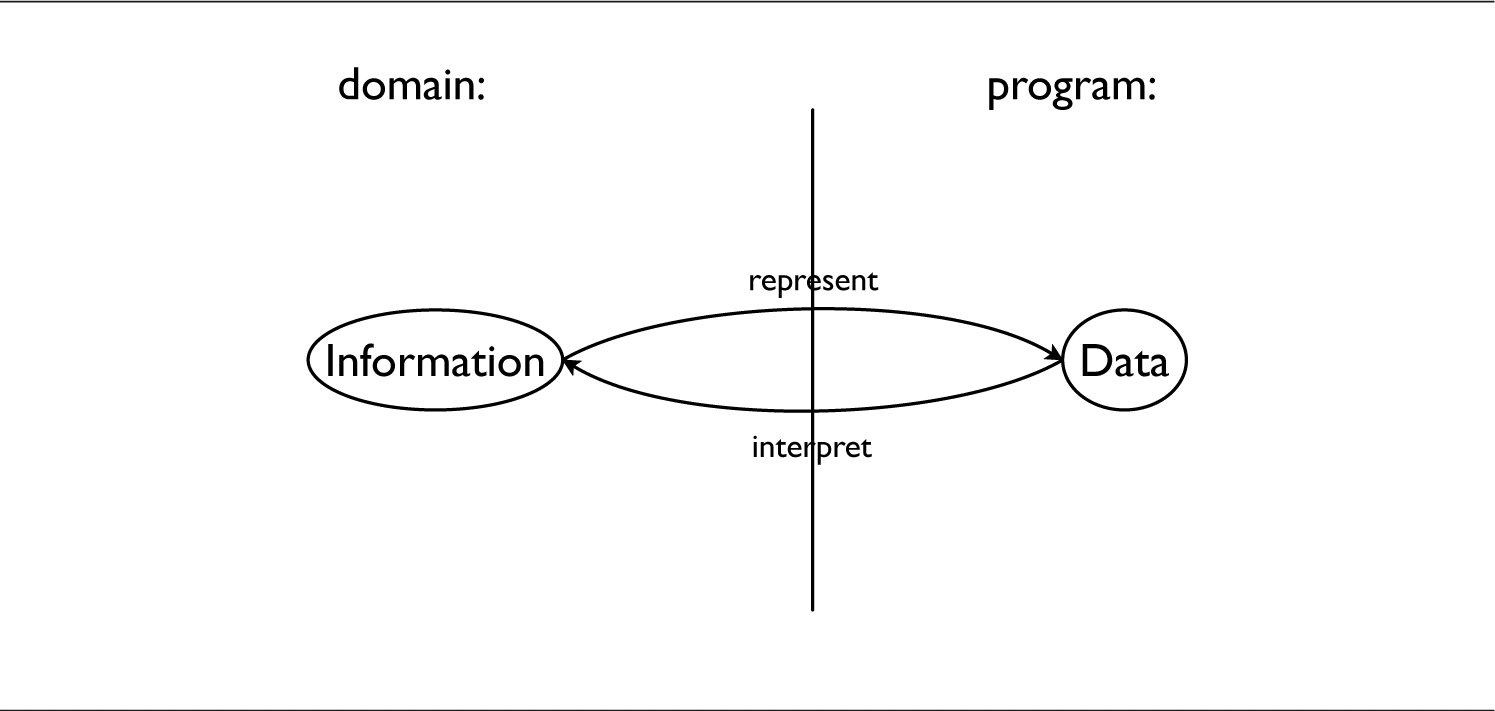
\includegraphics[width=0.75\textwidth]{images/00057.png}
  \caption{从现实领域信息到计算机数据，再由数据还原为领域信息}
  \label{fig:ch03_info_data}
\end{figure}

为了让这一核心概念生动具体，让我们考察几个现实场景。假设你正在设计一个以数值形式接收和产出信息的程序。尽管在计算机中选用数字作为底层数据表示极其简单，但如何\textbf{诠释}（interpretation）这些数据——即说明数值 42 在现实领域中到底代表什么——才是关键所在：
\begin{itemize}
  \item 在图像排版领域，42 可能代表距离画布顶端边界的像素偏移量；
  \item 在物理模拟或游戏世界中，42 可能代表动画精灵每个时钟周期移动的像素速率；
  \item 在气象物理领域，42 可能代表摄氏度、华氏度或开尔文温标下的测量温度；
  \item 在家具商城的库存系统中，42 可能代表某款餐桌的定制规格尺寸；
  \item 或者，42 仅仅代表某个文本字符串中的字符总数。
\end{itemize}
设计的精髓，就在于清晰掌握如何在现实信息与程序数据之间建立严谨、准确的双向映射桥梁。

鉴于这种认知映射对于每一位代码阅读者都至关重要，我们在代码中通过注释的形式将其明确记录下来，这被称为\term{数据定义}（data definitions）。数据定义承担着两大核心使命：
\begin{enumerate}
  \item 使用具有明确业务含义的词汇为某一类数据集合命名（赋予其一个数据类型名称）；
  \item 清晰告知代码阅读者如何创建属于该集合的有效数据，以及如何判断任意一个给定数据是否属于该数据类。
\end{enumerate}

\begin{notebox}[数据类 (Class)]
计算机科学家在这里使用“类”（Class）一词，其含义等同于数学中的“集合”（Set）。
\end{notebox}

下面是上述温度案例的一个规范数据定义示例：
\begin{lstlisting}[language=BSL]
; 一个 Temperature（温度）是一个 Number（数）。
; 诠释：代表摄氏度数值
\end{lstlisting}

第一行引入了该数据集合的专用名称 \code{Temperature}，并指明该类由全体数值（Number）构成。因此，当我们询问 102 是否是一个 Temperature 时，你可以笃定地回答“是”，因为 102 是一个数；同理，若问 \code{"cold"} 是否属于 Temperature，答案显然是“否”，因为字符串绝不属于数值。如果你被要求给出一个合法的 Temperature 样例，你可能会随手写出 $-400$。

如果你恰好掌握物理常识，知道现实宇宙中的理论最低温度（绝对零度）约为 $-273.15^\circ\text{C}$，你可能会好奇：我们能否在数据定义中精确表达这种物理现实约束？答案是完全可以！既然数据定义本质上是用严谨文本对数据集合的规范约定，你尽可以使用更精准的限制条件来定义温度。在接下来的章节中，我们将正式引入规范的区间与约束标记风格，例如“大于 $-273.15$ 的数”。

到目前为止，你已经见过了四种基础数据大类：\code{Number}、\code{String}、\code{Image} 以及 \code{Boolean}。在现阶段，制定一个新的数据定义，往往只是为已有的原生数据形态赋予一个贴合具体业务情境的新名字（例如将数值命名为温度）。即便仅凭这一点，也足以支撑起一套完整的函数设计配方。

\subsection{函数设计配方的六大步骤}

一旦明确了如何将输入的领域信息表示为计算机数据、以及如何将输出数据诠释为现实信息，设计单个函数的全过程就归纳为一套清晰、严密、环环相扣的标准配方：

\begin{recipebox}{函数设计配方 (Design Recipe for Functions)}
\begin{enumerate}
  \item \textbf{数据表示与数据定义 (Data Definition)}：明确现实信息如何表示为程序数据，写下核心数据定义与诠释注释。
  \item \textbf{签名、目的说明与函数头 (Signature, Purpose Statement, Header)}：
    \begin{itemize}
      \item \textbf{签名}（Signature）：指明函数消费什么类型的输入，产出什么类型的输出；
      \item \textbf{目的说明}（Purpose Statement）：用一两句话精炼阐释该函数计算的目标；
      \item \textbf{函数头 / 桩函数}（Header / Stub）：用形参变量搭建函数雏形，给出占位返回值。
    \end{itemize}
  \item \textbf{功能示例 (Functional Examples)}：根据签名选取典型输入，先于编码手工推导出预期的正确输出。
  \item \textbf{盘点资产与模板 (Inventory and Template)}：依据输入数据特征搭建函数体逻辑骨架，明确计算时可用的全部输入资产。
  \item \textbf{编写代码 (Coding)}：用具体的代数计算表达式填充模板，兑现目的说明中所承诺的业务契约。
  \item \textbf{自动化测试 (Testing)}：将先前的功能示例转化为可执行的单元测试，彻底验证函数的正确性。
\end{enumerate}
\end{recipebox}

让我们逐一深入剖析这六大步骤的具体实操：

\paragraph{第 1 步：数据表示与数据定义}
用单行注释或规范格式清晰声明数据表示方法。例如：
\begin{lstlisting}[language=BSL]
; 我们使用数（Number）表示以厘米为单位的长度。
\end{lstlisting}
为你认为对程序成功至关重要的核心概念拟定正式的数据定义。

\paragraph{第 2 步：签名、目的说明与函数头}
\term{函数签名}（Signature）是一条指引代码阅读者的核心注释，它清晰罗列了函数接收几个输入、这些输入分别来自哪些数据类、以及最终产出的数据属于什么类型。例如：
\begin{lstlisting}[language=BSL]
; String -> Number
; 接收一个字符串，产出其字符长度数值

; Temperature -> String
; 接收一个温度值，产出其状态描述文本

; Number String Image -> Image
; 接收一个数、一个字符串和一张图像，产出一张全新合成的图像
\end{lstlisting}

\term{目的说明}（Purpose Statement）是用简洁的一两行注释回答最本质的问题：\textbf{这个函数究竟计算出什么？} 任何阅读你代码的人，都应当无需通读复杂函数体，仅凭目的说明就能彻底洞悉函数的计算意图。

\term{函数头}（Header）又常被称为\term{桩函数}（Stub）：它确定函数名称，为签名中的每一个输入类别选取一个有意义的形参变量名，并在函数体中填入输出类别的任意一个默认字面量：
\begin{lstlisting}[language=BSL]
(define (f a-string) 0)
(define (g n) "a")
(define (h num str img) (empty-scene 100 100))
\end{lstlisting}
在编写目的说明时，善于利用形参变量名往往能让表达格外精准：
\begin{lstlisting}[language=BSL]
; Number String Image -> Image
; 将文字 s 绘制为图像并叠加到 img 上，
; 距顶部 y 像素，距左边缘 10 像素
(define (add-image y s img)
  (empty-scene 100 100))
\end{lstlisting}
至此，你已经可以点击【运行】按钮，语法检查会顺利通过。

\paragraph{第 3 步：功能示例}
通过列举具体生动的输入输出用例，来具象化签名和目的说明。从输入的合法数据集中挑选几个典型值，亲手计算出预期的正确答案：
\begin{lstlisting}[language=BSL]
; Number -> Number
; 计算边长为 len 的正方形的面积
; 给定输入: 2, 期望输出: 4
; 给定输入: 7, 期望输出: 49
(define (area-of-square len) 0)
\end{lstlisting}

\paragraph{第 4 步：梳理资产与模板}
在动手写实现之前，必须先\term{梳理已有资产}（take inventory，即盘点可用输入与组件）：我们手头拥有的已知输入是什么？需要计算出的目标又是什么？对于基础函数，所有已知数据均通过参数传入。为了时刻提醒自己这一核心事实，我们将桩函数中的虚拟默认值替换为一个包含所有形参变量的\term{模板}（template）：
\begin{lstlisting}[language=BSL]
(define (area-of-square len)
  (... len ...))
\end{lstlisting}
省略号 \code{(...)} 明确提醒你：这还不是一个能跑的代码，而是一张指明可用原料的结构图纸。

\paragraph{第 5 步：编写代码}
在 HtDP 体系中，所谓的“编码”（coding），就是用符合计算逻辑的具体表达式替换模板中的省略号，利用梳理出的已知参数与可用组件，彻底兑现目的说明中所许下的承诺：
\begin{lstlisting}[language=BSL]
; Number -> Number
; 计算边长为 len 的正方形的面积
; 给定: 2, 期望: 4
; 给定: 7, 期望: 49
(define (area-of-square len)
  (sqr len))
\end{lstlisting}
对于略复杂的函数（例如前文提到的 \code{add-image}），完成这一步需要组合多层图形绘制函数，如图~\ref{fig:ch03_step5} 所示。

\begin{figure}[htbp]
  \centering
\begin{lstlisting}[language=BSL, basicstyle=\scriptsize\ttfamily]
; Number String Image -> Image
; adds s to img, y pixels from top, 10 pixels to the left
; given:
;     5 for y,
;     "hello" for s, and
;     (empty-scene 100 100) for img
; expected:
;     (place-image (text "hello" 10 "red") 10 5 ...)
;     where ... is (empty-scene 100 100)
(define (add-image y s img)
  (place-image (text s 10 "red") 10 y img))
\end{lstlisting}
  \caption{函数设计第 5 步（编码兑现）的完成形态}
  \label{fig:ch03_step5}
\end{figure}

\paragraph{第 6 步：测试}
严谨设计的收尾之笔，是使用之前第 3 步列出的功能示例，对编写好的函数展开无情检验。点击运行，在交互区逐一验证：
\begin{replbox}
> (area-of-square 2)
4
> (area-of-square 7)
49
\end{replbox}

如果实际结果与预期完全一致，函数设计大功告成！若发生偏差，通常有三种可能原因：
\begin{enumerate}[label=(\alph*)]
  \item 你在第 3 步手工演算时粗心算错了预期值；
  \item 函数体代码编写有误，即程序存在逻辑缺陷（Bug）；
  \item 示例预期值与函数实现双双出现错误。
\end{enumerate}
排查时，应首先重新核验示例预期值的正确性；一旦确认示例无误，则全力排查函数体逻辑。


% ==============================================================================
% 3.2 基础练习：函数
% ==============================================================================
\section{基础练习：函数}
\label{sec:3.2}

接下来的几道基础练手习题与第~2.1~节中的练习题目高度相似，但请注意关键措辞的变化：第~2.1~节使用的是“定义”（define），而这里的要求全部是“\textbf{设计}”（design）！这意味着你必须\textbf{严格走完设计配方的全部六个步骤}，你的最终解答必须完整包含：数据定义、签名、目的说明、功能用例、模板及最终测试！

正如本节标题所示，这些练习是为了帮助你将设计配方内化为本能肌肉记忆。在这些步骤彻底变成你的第二本能之前，切勿跳过任何一步。编程世界中不乏极其深奥复杂的逻辑难题，我们绝不需要在低级疏忽上无谓浪费精力。

\begin{exercise}{设计提取首字符函数 string-first}{34}
严格按照设计配方，设计函数 \code{string-first}：从一个非空字符串中提取出它的第一个字符。暂时无需考虑空字符串的情况。
\end{exercise}

\begin{exercise}{设计提取尾字符函数 string-last}{35}
严格按照设计配方，设计函数 \code{string-last}：从一个非空字符串中提取出它的最后一个字符。
\end{exercise}

\begin{exercise}{设计计算图像面积函数 image-area}{36}
严格按照设计配方，设计函数 \code{image-area}：计算并返回给定图像所占据的像素总数（宽 $\times$ 高）。
\end{exercise}

\begin{exercise}{设计删除首字符函数 string-rest}{37}
严格按照设计配方，设计函数 \code{string-rest}：接收一个字符串，产出删除了首字符之后的其余字符串片段。
\end{exercise}

\begin{exercise}{设计删除尾字符函数 string-remove-last}{38}
严格按照设计配方，设计函数 \code{string-remove-last}：接收一个字符串，产出删除了末尾字符之后的其余字符串片段。
\end{exercise}


% ==============================================================================
% 3.3 领域知识
% ==============================================================================
\section{领域知识}
\label{sec:3.3}

初学者常会好奇：究竟需要具备怎样的知识储备，才能顺利写出函数体中的计算表达式？稍加审视便不难发现，这高度依赖于程序员对程序\term{业务领域}（domain）的认知深度。具体来说，领域知识主要来自两大方面：
\begin{enumerate}
  \item \textbf{外部应用领域的专业知识}：如数学、音乐、生物、土木建筑、金融或艺术等。程序员不可能通晓人类所有的行业学科，因此必须具备敏锐的跨界学习能力，能够听懂各行业专家的专业行话，并与之展开高密度的严谨讨论。数学往往是绝大多数理工领域的通用交集，但在更多交叉领域中，程序员必须边干边学。
  \item \textbf{所选编程语言及其标准库知识}：当任务涉及三角函数时，你需要知道 BSL 已经内置了 \code{tan}；当任务涉及图形绘制与动画渲染时，熟悉 \code{2htdp/image} 库的丰富接口将让你事半功倍。
\end{enumerate}

由于你永远无法预料未来会被委派去解决哪个领域的难题、或者必须使用哪一门编程工具，因此对可用计算工具箱的全貌建立清晰扎实的把握是生死攸关的。否则，那些略懂皮毛脚本的业务人员就会轻易取代你的位置。

通过审视设计配方第 1 步拟定的数据定义，你通常能一眼判断出该问题对领域知识的依赖程度：只要数据定义使用的是编程语言已经原生支持的数据形态，函数体的编写主要考验的是业务领域专业素养；而当我们在后文引入复杂自建数据结构时，程序设计的核心就转变为纯粹的计算机科学专业技能。


% ==============================================================================
% 3.4 从函数到程序
% ==============================================================================
\section{从函数到程序}
\label{sec:3.4}

真正的工程程序几乎不可能只由单体函数构成。大型系统不仅包含多重嵌套的函数网络，还包含广泛的全局常量定义。但无论软件系统多么宏大，系统化设计每一个基础函数的铁律绝不可动摇。

当你引入了全局常量后，各个函数都可以自由调用这些常量来计算结果。为了时刻提醒自己这些外部常量的存在，你可以把它们一并列入第 4 步的“资产盘点与模板”中作为可用资产。

多函数协作体系在交互式程序中表现得尤为明显：事件驱动系统天然需要专门处理键盘的函数、专门处理时钟的函数、以及负责图形渲染的视图函数。而在批处理程序中，拆分独立计算任务同样需要多个辅助函数的协同。这些子任务的需求，有时在阅读问题陈述之初就已浮出水面，有时则是在设计某一主函数的过程中中途顿悟发现的。

为此，我们强烈建议每一位开发者在纸上或代码注释中维护一张\term{愿望清单}（Wish List）。愿望清单上的每一个待实现条目均包含三项要素：
\begin{itemize}
  \item 一个见名知意的函数名称；
  \item 严谨清晰的函数签名；
  \item 简练的目的说明。
\end{itemize}

在设计批处理程序时，先将主函数放入愿望清单并开始攻坚；在设计交互式世界程序时，可将各个事件处理器、终止判断函数及场景渲染函数率先挂在愿望清单上。只要清单非空，就从中挑出一个愿望，运用六步设计配方彻底兑现它。如果在设计过程中发现需要新的辅助函数，立即将其追加到清单末尾。当清单上的所有愿望都被一一实现之时，整个程序便宣告完美竣工！


% ==============================================================================
% 3.5 关于测试
% ==============================================================================
\section{关于测试}
\label{sec:3.5}

手动执行测试很快就会沦为令人心力交瘁的苦力活。在交互区手工输入函数调用虽然直观，但要求肉眼反复校对复杂的数值或长文本。随着系统规模不断扩充，每次修改代码后都需要回归检验成百上千个用例，手动测试很快就会不堪重负，以至于程序员开始心存侥幸地怠慢测试。然而，严谨测试是捕捉并扑灭初级逻辑缺陷的第一道钢铁防线。马虎敷衍的测试必将迅速导致隐蔽 Bug 在代码库中潜伏滋生，最终全方位拖垮工程进度。

因此，\textbf{将测试全面自动化是现代软件工程的立身之本}！BSL 原生内置了极其优雅的自动化测试框架，DrRacket 会在后台全力保障其高效运行。让我们以华氏度转摄氏度的经典函数为例：
\begin{lstlisting}[language=BSL]
; Number -> Number
; 将华氏温度转换为摄氏温度
; 给定 32, 期望 0
; 给定 212, 期望 100
; 给定 -40, 期望 -40
(define (f2c f)
  (* 5/9 (- f 32)))
\end{lstlisting}

为了测试该函数，我们需要进行三次代数计算以及三次数值等值比较。在 BSL 中，你可以直接使用 \term{\code{check-expect}} 语法将其声明在定义区中：
\begin{lstlisting}[language=BSL]
(check-expect (f2c -40) -40)
(check-expect (f2c 32) 0)
(check-expect (f2c 212) 100)
\end{lstlisting}

现在只需轻轻点击【运行】按钮，DrRacket 就会自动运行并向你回报：\textbf{全套测试用例 100\% 全部通过！} 无需任何人工肉眼比对，省心省力！

当测试未通过时，\code{check-expect} 的威力表现得更为惊艳。假设我们故意在测试中引入一个错误断言：
\begin{lstlisting}[language=BSL]
(check-expect (f2c -40) 40)
\end{lstlisting}
再次点击运行，DrRacket 立即弹出一个专用的测试报告浮窗，清晰指出：3 个测试中有 1 个未通过，并以醒目的高亮对照列出：实际计算值（$-40$）、期望断言值（$40$），并附带可一键直达出错测试源码的超链接！

\code{check-expect} 既可以写在函数定义之后，也可以直接写在函数定义之前。点击运行后，DrRacket 会先预先加载所有函数定义，随后集中统一执行所有测试。如图~\ref{fig:ch03_testing} 所示，我们可以把设计配方的第 3 步（功能示例）与第 6 步（测试）合二为一：\textbf{直接用 \code{check-expect} 写出示例用例}。编写代码的同时就构筑好了测试护栏，未来对函数的任何微小修改，只需点击一次运行就能瞬间完成自动化回归验证。

\begin{figure}[htbp]
  \centering
\begin{lstlisting}[language=BSL, basicstyle=\scriptsize\ttfamily]
; Number -> Number
; converts Fahrenheit temperatures to Celsius temperatures

(check-expect (f2c -40) -40)
(check-expect (f2c 32) 0)
(check-expect (f2c 212) 100)

(define (f2c f)
  (* 5/9 (- f 32)))
\end{lstlisting}
  \caption{在 BSL 中运用 check-expect 构建自动化单元测试}
  \label{fig:ch03_testing}
\end{figure}

更令人拍案叫绝的是，\code{check-expect} 对图像对象完全原生支持！这意味着你可以直接对产出图像的视图函数展开像素级的精确断言。例如我们要设计小车渲染函数 \code{render}：
\begin{center}
  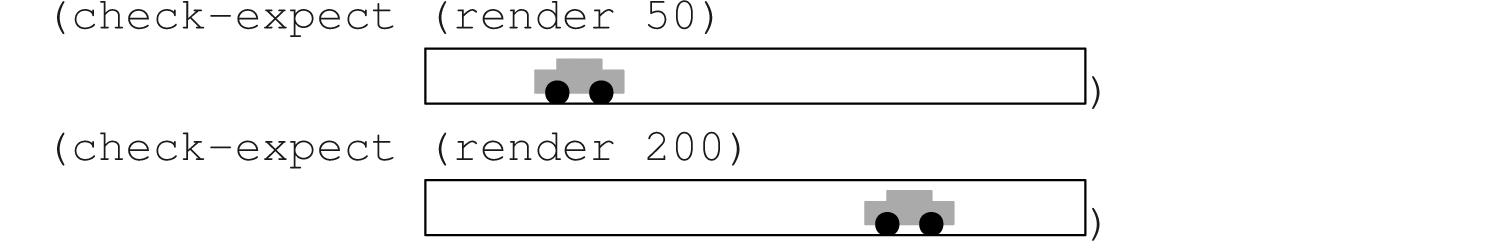
\includegraphics[width=0.85\textwidth]{images/00060.png}
\end{center}
或者，也可以使用绘图公式进行测试断言：
\begin{lstlisting}[language=BSL, basicstyle=\scriptsize\ttfamily]
(check-expect (render 50)
              (place-image CAR 50 Y-CAR BACKGROUND))
(check-expect (render 200)
              (place-image CAR 200 Y-CAR BACKGROUND))
\end{lstlisting}
后一种方式还能反哺指导我们推导函数体的具体实现逻辑。

这种由系统自动执行、针对独立软件组件开展的自动化测试机制被称为\term{单元测试}（Unit Testing）。在本书后续的所有章节中，我们将全面普及这种规范的测试实践。未来当你切换到其他主流编程语言时，你最先应该探索的也正是其对应的单元测试框架。


% ==============================================================================
% 3.6 设计世界程序
% ==============================================================================
\section{设计世界程序}
\label{sec:3.6}

前一章我们以探索性的方式介绍了 \code{2htdp/universe} 库；本节我们将展示如何将设计配方全面升华，系统化指导交互式“世界程序”的架构与设计。

世界程序库的核心运作理念非常清晰：开发者需要拟定一套代表整个“世界状态”的数据定义，以及一个能将任意世界状态绘制为可视画面的渲染函数 \code{render}。随后，根据应用需求设计响应时钟周期的 \code{tock}、响应键盘的 \code{key-handler} 以及响应鼠标的 \code{mouse-handler}；若需要在满足特定条件时退出，还需设计判定终止的谓词 \code{end?}。图~\ref{fig:ch03_wish_list} 给出了设计世界程序时标准的初始愿望清单蓝图。

\begin{figure}[htbp]
  \centering
\begin{lstlisting}[language=BSL, basicstyle=\scriptsize\ttfamily]
; WorldState: data that represents the state of the world (cw)

; WorldState -> Image
; when needed, big-bang obtains the image of the current
; state of the world by evaluating (render cw)
(define (render ws) ...)

; WorldState -> WorldState
; for each tick of the clock, big-bang obtains the next
; state of the world from (clock-tick-handler cw)
(define (clock-tick-handler cw) ...)

; WorldState String -> WorldState
; for each keystroke, big-bang obtains the next state
; from (keystroke-handler cw ke); ke represents the key
(define (keystroke-handler cw ke) ...)

; WorldState Number Number String -> WorldState
; for each mouse gesture, big-bang obtains the next state
; from (mouse-event-handler cw x y me) where x and y are
; the coordinates of the event and me is its description
(define (mouse-event-handler cw x y me) ...)

; WorldState -> Boolean
; after each event, big-bang evaluates (end? cw)
(define (end? cw) ...)
\end{lstlisting}
  \caption{设计交互式世界程序的通用初始愿望清单}
  \label{fig:ch03_wish_list}
\end{figure}

让我们通过一个生动的实战案例来完整演练这套设计配方：

\begin{notebox}[案例实战：小车水平匀速行驶]
\textbf{问题陈述}：设计一个动画世界程序，使一辆小车在画布场景中从左向右持续平移，每经历一个时钟周期向右移动 3 个像素。
\end{notebox}

对于这个场景，我们可以直观勾勒出不同时刻的世界画面：
\begin{center}
  
\includegraphics[width=0.85\textwidth]{images/00063.png}
\end{center}

世界程序的设计配方包含三大核心阶段外加一个装配步骤：

\begin{recipebox}{世界程序设计配方 (Design Recipe for World Programs)}
\begin{enumerate}
  \item \textbf{界定并提取全局常量}：
    \begin{itemize}
      \item \textbf{物理常量}：描述世界中物体的固有属性（运动速度、宽高、车轮半径等）；
      \item \textbf{图形常量}：在画布上静态呈现的各种基础视觉元素（车轮、车身、树木、背景等）。
    \end{itemize}
  \item \textbf{确立世界状态的数据表示 (WorldState)}：辨识随着时间推移、受事件驱动而动态改变的核心属性，为其拟定精确的数据定义与业务诠释。
  \item \textbf{逐一兑现愿望清单上的各个处理函数}：
    \begin{itemize}
      \item 必备的场景渲染函数 \code{render : WorldState -> Image}；
      \item 按需设计时钟、键盘、鼠标事件处理器及终止判定谓词。
    \end{itemize}
  \item \textbf{编写主启动函数 (main)}：将初始状态与各事件子句装配进 \code{big-bang} 表达式中。
\end{enumerate}
\end{recipebox}

\paragraph{第一步：常量抽取与单点控制原则}
在小车行进世界中，小车运动速率、画布长宽以及车轮间距是恒定不变的“物理常量”：
\begin{lstlisting}[language=BSL]
(define WIDTH-OF-WORLD 200)
(define WHEEL-RADIUS 5)
(define WHEEL-DISTANCE (* WHEEL-RADIUS 5))
\end{lstlisting}

进而，我们可以通过代数运算由物理常量派生构建小车的各部分“图形常量”：
\begin{lstlisting}[language=BSL]
(define WHEEL (circle WHEEL-RADIUS "solid" "black"))
(define SPACE (rectangle ... WHEEL-RADIUS ... "white"))
(define BOTH-WHEELS (beside WHEEL SPACE WHEEL))
\end{lstlisting}

\begin{exercise}{单点控制原则与汽车图像缩放}{39}
优秀的软件架构师会确保像 \code{CAR} 这样的复杂图形常量能够通过修改单个底层基准常量来实现全局等比缩放。我们在构建小车时以车轮半径为基准：
\begin{lstlisting}[language=BSL]
(define WHEEL-RADIUS 5)
\end{lstlisting}
所有车轮间距、车身长宽、车顶弧度均以此为依据派生计算。这样一来，将 \code{WHEEL-RADIUS} 从 5 改为 10，整辆小车就会全局自适应等比放大一倍。这种卓越的工程规范被称为\term{单点控制原则}（single point of control）。请设计并绘制一辆你喜欢的小汽车图像，确保 \code{WHEEL-RADIUS} 是控制其尺寸的唯一控制源。
\end{exercise}

\paragraph{第二步：世界状态数据定义}
在动画播放过程中，动态演变的是小车相对于场景左边界的距离。距离可以用非负数值精确刻画，因此我们写下清晰的数据定义：
\begin{lstlisting}[language=BSL]
; 一个 WorldState 是一个 Number。
; 诠释：代表小车距离画布左边界的像素位移量
\end{lstlisting}

\paragraph{第三步：愿望清单与函数设计}
根据业务规则，我们需要一个时钟处理器 \code{tock}（每次时钟周期小车右移 3 像素）和一个渲染函数 \code{render}：
\begin{lstlisting}[language=BSL]
; WorldState -> WorldState
; 每次时钟滴答，将小车横坐标加 3
(check-expect (tock 20) 23)
(check-expect (tock 78) 81)
(define (tock ws)
  (+ ws 3))
\end{lstlisting}

\begin{exercise}{将样例改写为 BSL 自动化测试}{40}
将上述 \code{tock} 函数的示例在 DrRacket 中编写为完整的 \code{check-expect} 测试。故意在测试中制造一个计算偏差，观察自动化测试窗口的报错交互反馈；随后将其修正并重新运行。
\end{exercise}

接下来设计视图渲染函数 \code{render}。我们可以通过图~\ref{fig:ch03_car_examples} 中的对照表格来直观归纳函数体的构造规律：
\begin{figure}[htbp]
  \centering
  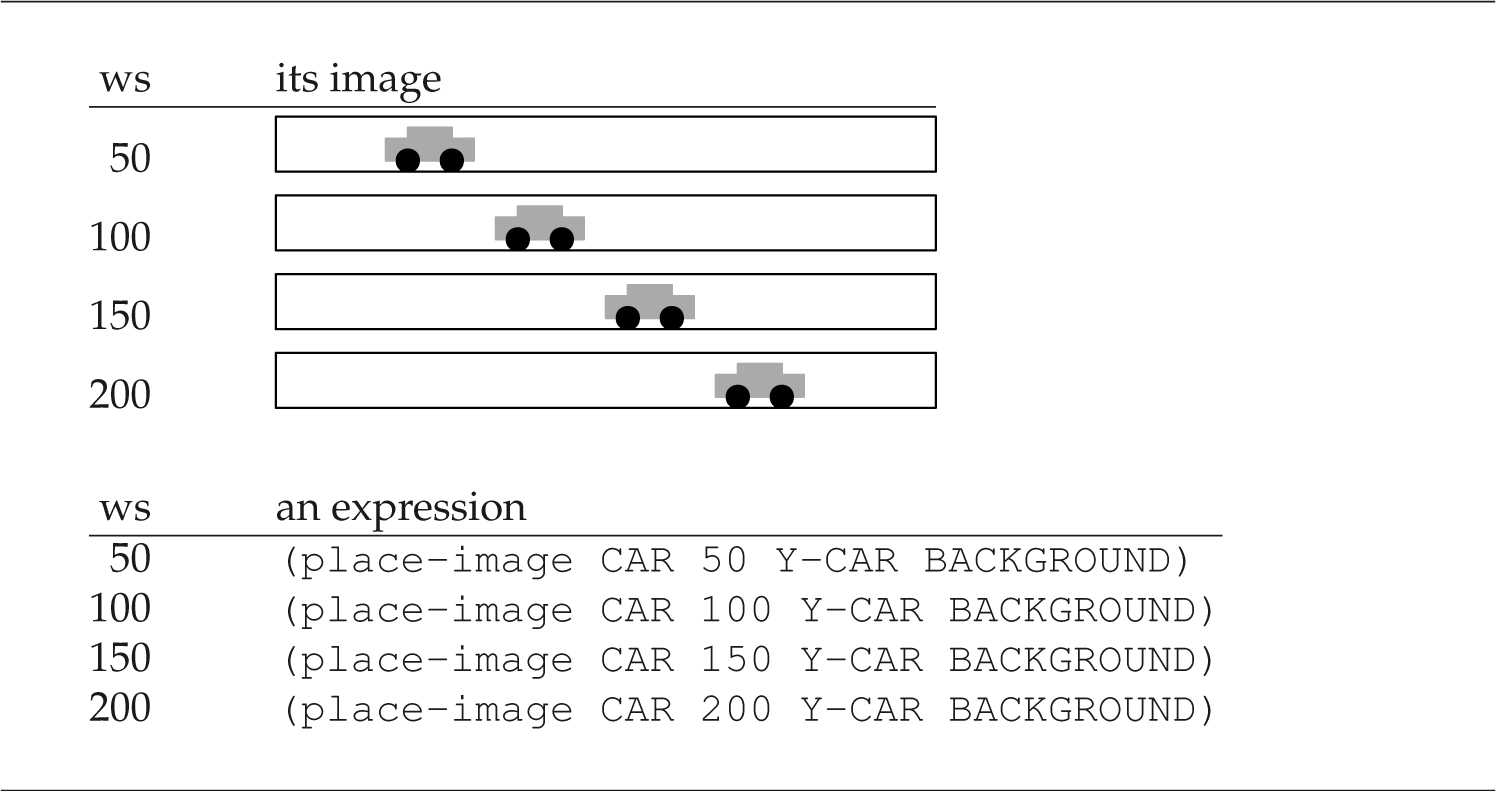
\includegraphics[width=0.85\textwidth]{images/00065.png}
  \caption{小车移动程序的视觉用例与代数表达式构造}
  \label{fig:ch03_car_examples}
\end{figure}

由此水到渠成地完成 \code{render} 的实现：
\begin{lstlisting}[language=BSL]
; WorldState -> Image
; 将小车按照当前状态 ws 绘制到背景画布 BACKGROUND 上
(define (render ws)
  (place-image CAR ws Y-CAR BACKGROUND))
\end{lstlisting}

\paragraph{第四步：编写 main 函数并点火运行}
将所有零件齐备后，主函数只需负责把初始状态和事件蓝图组装进 \code{big-bang} 中：
\begin{lstlisting}[language=BSL]
; WorldState -> WorldState
; launches the program from some initial state
(define (main ws)
   (big-bang ws
     [on-tick tock]
     [to-draw render]))
\end{lstlisting}

在交互区执行 \code{(main 13)}，你就能亲眼见证一辆小汽车从距左边缘 13 像素处平稳匀速驶向屏幕右侧！

\begin{exercise}{组装运行小车动画并添加树木背景}{41}
在完成练习~\ref{ex:39} 的基础上，定义 \code{BACKGROUND} 和 \code{Y-CAR} 常量，将上述所有函数组装成完整程序并在 DrRacket 中顺利运行。程序运转正常后，为背景增添一棵生动的绿树作为点缀。例如可以使用以下代码组合出一棵小树：
\begin{lstlisting}[language=BSL]
(define tree
  (underlay/xy (circle 10 "solid" "green")
               9 15
               (rectangle 2 20 "solid" "brown")))
\end{lstlisting}
此外，在 \code{big-bang} 中增加一个 \code{stop-when} 子句，使小汽车在完全开出右边界时自动优雅停止。
\end{exercise}

\begin{exercise}{修改状态诠释：小车右侧边缘坐标}{42}
修改上述数据定义的业务诠释：让世界状态 \code{WorldState} 表示小汽车\textbf{最右侧边缘}所在的横坐标位置。审视并重新调整你的渲染与判断逻辑。
\end{exercise}

\begin{exercise}{基于时间的动画状态设计与正弦运动}{43}
让我们用另一种极富洞见的视角重新审视上述问题：将世界状态定义为动画启动以来所经历的\textbf{绝对时钟滴答次数}：
\begin{lstlisting}[language=BSL]
; 一个 AnimationState 是一个 Number。
; 诠释：表示动画启动以来累计流逝的时钟滴答周期数
\end{lstlisting}
重新设计 \code{tock} 与 \code{render} 函数。进一步发挥数学魅力：利用三角函数 \code{sin} 设计一个小车沿着正弦波上下起伏前行的趣味动画世界！
\end{exercise}

\subsection{响应鼠标与超空间跃迁}

通过引入鼠标事件处理，我们能进一步体会“模型与视图彻底分离”所带来的无与伦比的架构弹性：
\begin{notebox}[案例拓展：超空间瞬间跃迁]
在原有小车匀速右移的基础上增加新特性：当用户在画布任意位置点击鼠标时，小汽车瞬间“跃迁”移动到该鼠标点击处的横坐标位置！
\end{notebox}

面对这一业务拓展，设计配方为我们提供了清晰的演进罗盘：
\begin{enumerate}
  \item 没有新增物理量，现有常量库无需变更；
  \item 动态演进的仍然只是小车的横坐标，现有数据定义 \code{WorldState} 依然完美适用；
  \item 唯一需要新增的，是处理鼠标点击的愿望条目：
\begin{lstlisting}[language=BSL]
; WorldState Number Number String -> WorldState
; 若鼠标事件 me 为 "button-down"，则将小车瞬间转移到 x-mouse 处
(define (hyper x-position-of-car x-mouse y-mouse me)
  x-position-of-car)
\end{lstlisting}
  \item 在主函数 \code{main} 的 \code{big-bang} 中直接追加一行 \code{[on-mouse hyper]} 即可：
\begin{lstlisting}[language=BSL]
(define (main ws)
  (big-bang ws
    [on-tick tock]
    [on-mouse hyper]
    [to-draw render]))
\end{lstlisting}
\end{enumerate}

接下来只需运用函数设计配方兑现 \code{hyper} 函数：
\begin{lstlisting}[language=BSL]
; WorldState Number Number String -> WorldState
; 鼠标点击处理函数
; 示例：
; 给定: 21 10 20 "enter",       期望: 21
; 给定: 42 10 20 "button-down", 期望: 10
; 给定: 42 10 20 "move",        期望: 42
(define (hyper x-position-of-car x-mouse y-mouse me)
  x-position-of-car)
\end{lstlisting}

\begin{exercise}{为鼠标事件编写 BSL 单元测试}{44}
将上述 \code{hyper} 函数的三个功能示例转化为正式的 \code{check-expect} 测试用例。在尚未写出实现之前运行，亲眼见证测试如期失败。
\end{exercise}

随后使用条件分支 \code{cond} 实现该函数：
\begin{lstlisting}[language=BSL, basicstyle=\scriptsize\ttfamily]
; WorldState Number Number String -> WorldState
; places the car at x-mouse
; if the given me is "button-down"
(define (hyper x-position-of-car x-mouse y-mouse me)
  (cond
    [(string=? "button-down" me) x-mouse]
    [else x-position-of-car]))
\end{lstlisting}
再次点击运行，测试全部通过！执行 \code{(main 1)}，尽情享受鼠标遥控小车瞬间跃迁的超快感！


% ==============================================================================
% 3.7 虚拟宠物世界
% ==============================================================================
\section{虚拟宠物世界}
\label{sec:3.7}

本节的综合项目练习将带领大家构建一个经典的电子虚拟宠物（Virtual Pet）游戏原型。我们的小猫会在画布上持续漫步前行；然而孤独漫步会让小猫逐渐感到失落不开心。正如真实宠物一样，你可以尝试抚摸小猫（提升一点快乐度），或者给它喂食小鱼干（让它超级开心满足）！

首先在代码中定义我们钟爱的小猫形象：
\begin{stepperbox}
\begin{Verbatim}[commandchars=\\\{\}, fontsize=\footnotesize]
(define cat1 \inlinesprite[2.2em]{images/sprites/cat1.png})
\end{Verbatim}
\end{stepperbox}

\begin{exercise}{虚拟宠物：循环移动的小猫}{45}
设计一个名为 \code{cat-prog} 的世界程序，让小猫以每个时钟周期 3 个像素的速度在屏幕上自左向右匀速漫步。该程序接收小猫的初始横坐标作为启动参数。当小猫从右侧边缘完全走出屏幕时，它能像环游世界一样，瞬间从最左侧边界重新出现并循环行进。

\textbf{提示：}查阅 DrRacket 帮助文档中的取模函数 \code{modulo}，思考它如何帮助实现无缝循环。
\end{exercise}

\begin{exercise}{双帧交替步态动画}{46}
为了让小猫的步伐更加生动逼真，我们准备了另一张迈出不同步伐的小猫图片：
\begin{stepperbox}
\begin{Verbatim}[commandchars=\\\{\}, fontsize=\footnotesize]
(define cat2 \inlinesprite[2.2em]{images/sprites/cat2.png})
\end{Verbatim}
\end{stepperbox}
修改练习~\ref{ex:45} 中的渲染函数：根据当前小猫横坐标数值是奇数还是偶数，交替选用两张不同姿态的小猫图片（查阅文档中的 \code{odd?} 谓词），从而呈现出生动连贯的漫步动画！
\end{exercise}

\begin{exercise}{虚拟宠物：设计快乐度计量表}{47}
设计一个独立的世界程序 \code{gauge-prog}，用来实时维护并显示宠物的“快乐度计量表”（happiness gauge）。程序接收初始最大快乐度数值。计量表以满分状态起步，随时间推移，每个时钟周期快乐度自然衰减 0.1；但无论如何衰减，快乐度最低不会跌破 0 分下限。

当玩家按下键盘上的【向下方向键】时，快乐度增加满分的 $1/5$；而每次按下【向上方向键】（代表喂食美味罐头），快乐度瞬间跳升满分的 $1/3$！

快乐度通过场景中央一个带有黑色外框的红色实心矩形进度条直观呈现：快乐度为 0 时红条消失；达到满分 100 时红条完整横跨画布。
\end{exercise}

\vspace{1em}
\begin{notebox}[更宏大的宠物世界愿景]
随着你在后续章节学到更多高阶复合数据结构，我们将向你揭示如何把练习~\ref{ex:45} 的行走小猫与练习~\ref{ex:47} 的心情仪表盘完美合体：漫步的小猫若长久无人理会就会日益沮丧；而当你抚摸它、喂饱它时，它会瞬间欢呼雀跃！这也是为什么在学完这前三章后，你必定会迫不及待地渴望探索更广阔程序设计世界的原因！
\end{notebox}
